% Method Section - Concise NeurIPS style

\begin{figure}[t]
\centering
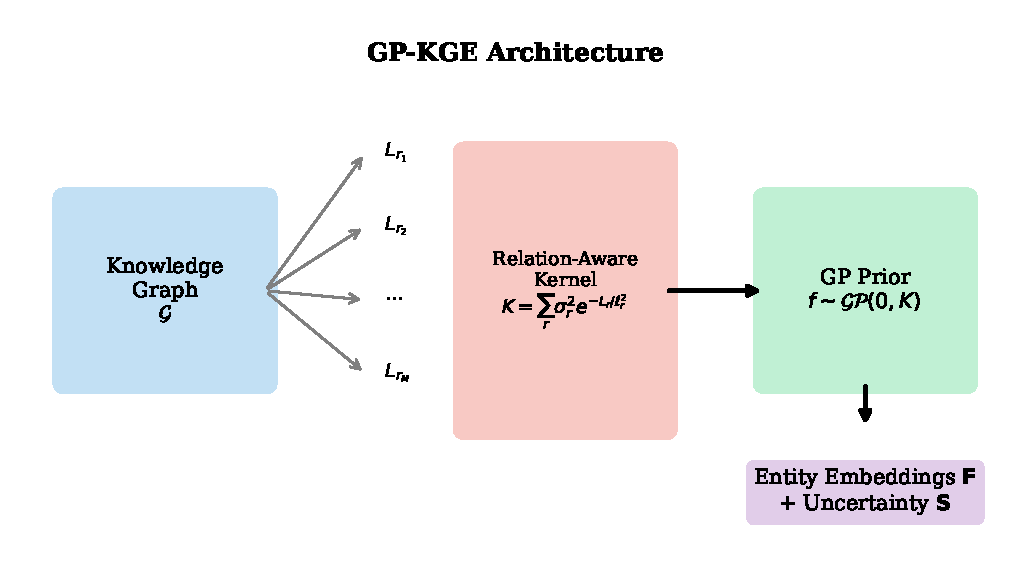
\includegraphics[width=0.95\linewidth]{figures/architecture.pdf}
\caption{\ours{} architecture: Per-relation Laplacians define a relation-aware kernel for the GP prior over entity embeddings.}
\label{fig:architecture}
\end{figure}

\subsection{Problem Setup}

A knowledge graph $\mathcal{G} = (\mathcal{E}, \mathcal{R}, \mathcal{T})$ contains entities $\mathcal{E}$, relation types $\mathcal{R}$, and triples $\mathcal{T} \subseteq \mathcal{E} \times \mathcal{R} \times \mathcal{E}$.
We learn entity embeddings $\mat{F} \in \R^{N \times d}$ that are (1) predictive for link prediction and (2) equipped with calibrated uncertainty estimates reflecting graph structure.

\subsection{Relation-Aware Kernel}

For each relation $r$, let $\mat{L}_r = \mat{I} - \mat{D}_r^{-1/2}\mat{A}_r\mat{D}_r^{-1/2}$ be the normalized Laplacian of the relation-$r$ subgraph.
Our kernel aggregates relation-specific diffusion processes:
\begin{equation}
    \mat{K} = \sum_{r=1}^{M} \sigma_r^2 \cdot \exp\left(-\frac{\mat{L}_r}{\ell_r^2}\right)
    \label{eq:kernel}
\end{equation}
where $\sigma_r^2$ controls relation $r$'s contribution and $\ell_r$ controls information propagation distance.
The kernel is computed via eigendecomposition: $\exp(-\mat{L}_r/\ell_r^2) = \mat{U}_r \exp(-\mat{\Lambda}_r/\ell_r^2) \mat{U}_r^\top$.

\begin{proposition}
$\mat{K}$ is positive semi-definite (valid kernel).
\end{proposition}
\begin{proof}
Each $\mat{L}_r$ is PSD $\Rightarrow$ $\exp(-\mat{L}_r/\ell_r^2)$ is PSD $\Rightarrow$ weighted sum with $\sigma_r^2 > 0$ is PSD.
\end{proof}

\subsection{GP Prior and Variational Inference}

We place independent GP priors per embedding dimension:
$\vect{f}^{(j)} \sim \GP(0, \mat{K})$ for $j = 1, \ldots, d$.
For link prediction, we use DistMult scoring: $s(h,r,t) = \langle \vect{f}_h, \vect{w}_r, \vect{f}_t \rangle$.

We approximate the posterior with $q(\mat{F}) = \N(\mat{M}, \mat{S})$ and maximize the ELBO:
\begin{equation}
    \mathcal{L} = \E_{q}[\log p(\mathcal{T} | \mat{F})] - \beta \cdot \KL(q(\mat{F}) \| p(\mat{F} | \mat{K}))
\end{equation}
For scalability, we use $P$ inducing points, reducing complexity from $O(N^3)$ to $O(NP^2 + P^3)$.

\subsection{Entity-Level Uncertainty}

The posterior variance $\mat{S}_{ii}$ quantifies uncertainty for entity $e_i$.
For a query $(h, r, t)$, prediction uncertainty propagates through the scoring function:
\begin{equation}
    \text{Var}[s(h,r,t)] \approx \sum_{i} w_{r,i}^2 (S_{hh,i} m_{t,i}^2 + S_{tt,i} m_{h,i}^2 + S_{hh,i} S_{tt,i})
\end{equation}
High uncertainty flags potentially unreliable predictions, enabling OOD detection.
